\chapter{InterSCSimulator}
\label{cap:interscsimulator}

In this chapter, we will present InterSCSimulator, an open-source, large-scale Smart City simulator. The goal of this simulator is to simulate complex Smart Cities scenarios with millions of agents. The current version of the software allows the simulation of different traffic scenarios. Section \ref{sec:simulacaoRequisitos} describes the functional and non-functional requirements handled in the simulator implementation. Section \ref{sub:architecture} presents the architecture of the simulator. Section \ref{sub:modelo} describes the implementation of the traffic model used in the simulator. Section \ref{sub:components} presents the inputs, outputs, and components of the simulator. Section \ref{sec:outros} lists extensions to the simulator to allow the simulation of other Smart City applications domains, some of them already implemented. Finally, Section \ref{sec:evolucao} describes the evolution and challenges faced during the simulator implementation.

\section{InterSCSimulator Requirements}
\label{sec:simulacaoRequisitos}

In this section, we will describe all the requirements handled in the InterSCSimulator implementation. 

\subsection{Functional Requirements}
\label{subsec:requirements}

To identify the functional requirements of InterSCSimulator, we studied the simulators presented in Chapter \ref{cap:relacionados} and the Smart City domains presented in Chapter \ref{cap:conceitos}. In this work, we decided to focus on the mobility domain because it has important challenges and is related to many other city domains such as health and garbage collection.

The main functional requirements are the representation of the road network of the city, the definition of simulated travels and a model to allow realistic movement in the city. The list of the requirements is in the following:

\begin{itemize}

\item \textbf{Road Network Representation: } In a Smart City simulator, it is necessary to represent a real city network to allow the simulation of the movement of vehicles and people in the city. This network must be described in a data structure easy to manipulate and execute algorithms such as to find the best path and calculate vehicles speed. The approach used by most simulators is creating a digraph of the city using a map from a map service such as Google Maps\footnote{Google Maps - \url{googlemaps.com}} or Open Street Maps\footnote{Open Street Maps - \url{www.openstreetmap.org}}.

\item \textbf{Travels Definition: } The simulator must receive a list of travels that it must simulate with parameters such as origin, destination, and travel time. There are many possibilities to create the travels such as an Origin-Destination (OD) survey \cite{khan2016accurately}, real mobility traces from smartphones \cite{jamil2014crowdsensing}, and random travels. In this work, we created tools to convert the OD created by the municipality of S\~ao Paulo to the format of our simulator.

\item \textbf{Vehicle Simulation: } It is necessary to define a mathematical model to calculate the flow and speed of the vehicles. There are many models available in the literature, from a very complex micro-model to a very simple free-flow model. This work uses a mesoscopic model described by Song. et al. \cite{song2017gpusimulation} and will be detailed in Section \ref{sub:modelo}.

\item \textbf{Pedestrian Simulation: } Besides the vehicles, it is necessary to model pedestrian movements to allow movements to subway stations and bus stops and also trips made entirely on foot. 

\item \textbf{Bus System: } It is necessary to model bus stops and bus trips, allowing passengers to enter and leave the vehicles. The buses must move on the city using the same traffic model used by the car simulation. 

\item \textbf{Subway: } To simulate big cities, it is also necessary to model the subway network of the town, allowing commuters to arrive at the stations by all the other travel modes.

\item \textbf{Simulation Output: } The simulator must generate outputs to allow data analyses and visualization of the simulation. Typically, the simulators create a trace file with all the events occurred during the simulation. Our simulator also saves a trace file in XML or CVS format.

\item \textbf{Data Analyses: } The simulator output must facilitate the data analyzes using statistical tools such as R and Python. Hence, all the output must have all the crucial events of the simulation.

\item \textbf{Simulation Visualization: } The simulator also must allow an animated visualization of the simulation. Many simulators already have an integrated tool to visualize the simulation during execution time, and other have a tool that analyzes the simulation output and generates the visualization.

\end{itemize}

The requirements show that the simulator must receive as inputs the road network of a city and the list of travels that will be simulated. Other possible data is information about public transportation and pedestrians. With this data, the simulator must calculate the agents travel using different mobility models. Finally, the simulator must save the events to allow the data visualization and analyses.

\subsection{Non-Functional Requirements}
\label{sec:nonfunctional}

Besides the functional requirements, a Smart City simulator must also (1) allow the easy definition of the simulation scenarios, (2) allow the execution of scenarios with millions of simultaneous actors, and (3) allow the easy extension of the simulator. Therefore, the non-functional requirements handled by the simulator are:

\begin{itemize}

\item \textbf{Scalability: } To simulate an entire city, it is necessary to manage millions of simultaneous actors such as cars, people, sensors, and building. Therefore, the simulator must scale from hundreds to millions of actors. To achieve this objective, it is required the use of efficient algorithms and data structures and the development of a massively parallel and distributed simulator.

\item \textbf{Usability: } The definition of a simulation scenario must be simple, allowing people that are not computer specialist use the simulator without knowing its internal implementation. Most of the analyzed simulators use XML files to the definition of the scenarios, many of them provide tools to convert data from different sources to the format of the simulator such as maps, origin-destination matrix, and bus lines.

\item \textbf{Extensibility: } It is highly unlikely that a simulator provides all the models and abstractions required to create all the Smart City simulations. Therefore, the extension of the simulator must be straightforward, offering simple mechanisms to allow the implementation of new actors and the extension of the existing ones. It is an excellent vantage of open source simulators that has a well-documented architecture and code.

\end{itemize}

\section{Simulator Architecture}
\label{sub:architecture}

InterSCSimulator has a three-layer architecture. Figure \ref{fig:arquitetura} presents the layers: \textbf{Sim-Diasca} is a generic, discrete-event simulator that offers the necessary tools to develop simulator models, \textbf{City Model} which implements the behavior of the city actors and is the central part of this work and \textbf{Simulation Scenarios} which are the possible simulation scenarios developed with the city model.

\begin{figure}[!htb]
\centering
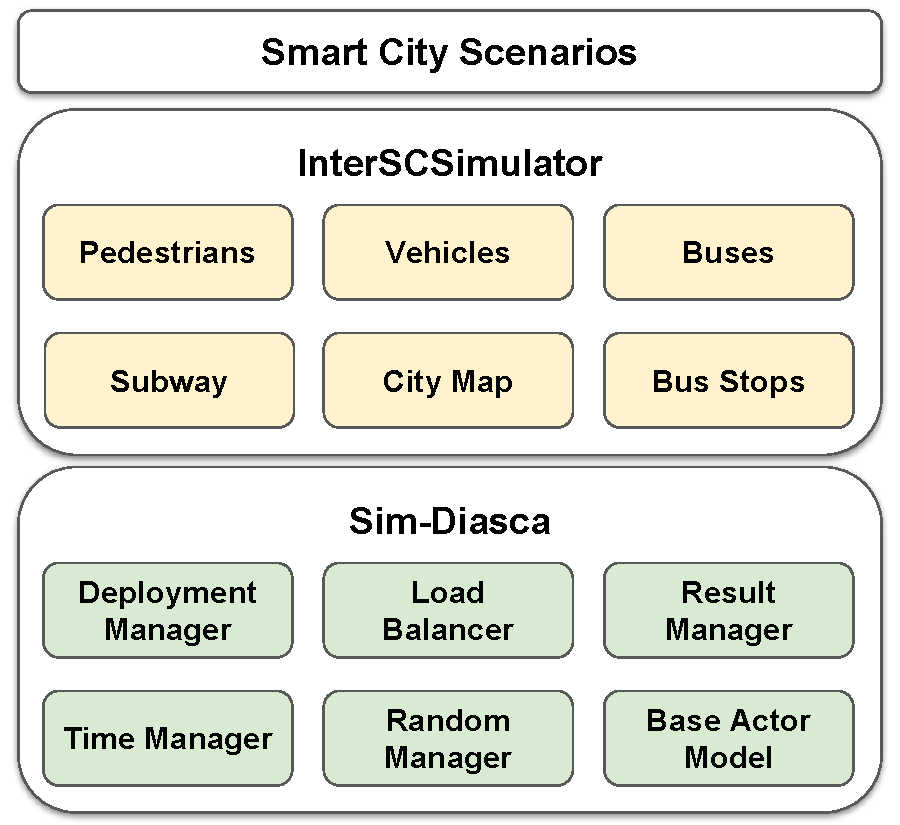
\includegraphics[width=0.9\textwidth]{figuras/chap-interscsimulator/Architecture.pdf}
\caption{InterSCSimulator Architecture}
\label{fig:arquitetura}
\end{figure}

Sim-Diasca main requirements are the simulation time management, the random number generation (allowing reproducibility), the synchronization of the actors to guarantee the simulation consistency and a basic actor model to facilitate the development of the simulation model. Besides, using the Erlang language, Sim-Diasca facilitates the communication among the actors, the parallelism, and distribution of the simulator, and fault tolerance.

The City Model is composed of the actors that are simulated in the Smart City scenarios. This layer is the central development of this research. The current version of the simulator provides the following actors: \textbf{Person} that represents a person traveling in the city, \textbf{Car}, when a person travels in a car, \textbf{Bus}, that represents the buses moving in the city and allow the boarding of passengers, \textbf{Subway} that simulates the subway network of the city, \textbf{Sensor} to reproduce Smart City sensors. Besides the actors, there are many other structures in the model, such as the city graph representation, an API to retrieve real-time simulation data, and a structure to save the simulation event log.

\section{Mobility Models}
\label{sub:modelo}

InterSCSimulator has many models to simulate the mobility of a city population, including a traffic model, which calculates the speed of the vehicles in the streets, a simple pedestrian model, and a model to simulates public transportation travels by subway or buses. A person can also make a trip using different travel modes, for example, the person starts walking to a subway station, then makes subway travel, and finally, get a bus to reach his destination. The next subsections describe the main models used by the simulator.

\subsection{Vehicles Simulation}

Car travels are composed of a sequence of links that the car will pass. To calculate the speed of the car in each link, the InterSCSimulator uses a mesoscopic traffic model. This type of model simulates each car individually. However, the speed of these vehicles is calculated using a density function relating to the capacity of the street and the number of vehicles on the street \cite{song2017gpusimulation}. The model implemented uses the following density function:

\[
v=v0*(( 1 - ( \frac{k}{k_{jam}} ) ^ \beta ) ) ^ \alpha
\]

Where:

\begin{itemize}

\item $v0$: the maximum speed of the street, used when the street is not congested.
\item k: the current street density.
\item kjam: the density when the street is congested.
\item $\alpha$ e $\beta$: Configurable parameters that are defined by the calibration of the model. We used the values used in the original paper $\alpha$=1.0 and $\beta$=0.05. 

\end{itemize}

This function is always used when a vehicle enters in an edge of the graph. To calculates its speed, it is verified the current density in the edge and using the function, the speed is calculated. With the speed and the length of the edge, it is possible to calculate the time that the will need to go through the edge. The time is calculated using the following function:

\[
time = \frac{edge\_length}{vehicle\_speed}
\]

In the function, \textbf{time} is the seconds that the car takes to go through the edge, \textbf{vehicle\_speed} is the value calculated by the traffic model and represents the speed (m/s) of the car in the street, and  \textbf{edge\_length} is the street length (m) that is available at OpenStreetMaps.


\subsection{Pedestrian Simulation}

Pedestrian simulation resembles the vehicle simulation. However, the speed calculus is straightforward. We used a normal distribution with mean 1.2 m/s, and a random speed calculated to the person. The function used to calculate the time that a person will take to go through an edge is the same used by the vehicles.

\subsection{Subway Simulation}

To simulate the subway system, InterSCSimulator has the subway graph of the simulated city, and it calculates the travel time of the subway travel by the number of stations that separate the origin and destination stations of the trip. Commonly, city documents with the subway system describe the travel duration between two following stations. Hence, we use a fixed time to calculate the travel time of the person in the subway system.

When an agent arrives at the origin subway stations, it sends a message to an Erlang process which simulates the subway system with its destination station. The Erlang process calculates the time that the agent will spend in the subway system, and then the person waits this time. After this interval, the agent is moved to the destination station and can finish its travel.

\subsection{Bus Trip Simulation}

The buses are simulated using the same traffic model used by the cars. The difference is that the buses pass in a sequence of links that represent bus stops. The people in the bus stop can board the bus if the line of the bus is the same that they are waiting.

The person can go walking or by car from its origin until a nearby bus stop. In the bus stop, the person waits for a bus of his desired line. When the bus arrives, the person boards the bus and moves using the same path and speed of the bus. When the bus comes at the destination bus stop, the person outboards the vehicle and the person finishes his travel.

The buses can have a maximum of 75 passengers, which is the limit of the city of S\~ao Paulo\footnote{http://goo.gl/B7NJbj}. 

\subsection{Multimodal Travels}

The simulator allows a sequence of travels using the same or different travel modes. To this, each person can have a series of trips and the destination of each travel is the origin of the next one. Each travel does not have any relation to the previous one. However, the final attributes of the journey such as total time traveled distance, and travel cost is the sum of all travels.

\section{Simulator Components}
\label{sub:components}

InterSCSimulator has three main components: \textbf{Scenario Definition} which read the input files and creates the simulation scenarios. \textbf{Simulator Engine} responsible for executing the algorithms and models of the simulation. \textbf{Events Manager} that receives all the events occurred in the simulation and saves in the trace file or send to the real-time API.

At the end of the simulation, there are other two components based on the result simulation: \textbf{Animated Visualization} which allows the graphic visualization of the events in the city graph and \textbf{Output Analyses} that using the output data perform statistical analyses using scripts R. Figure \ref{fig:simComponents} presents the simulator components, the interactions among them, and the simulator input and output files.

\begin{figure}[!htb]
\centering
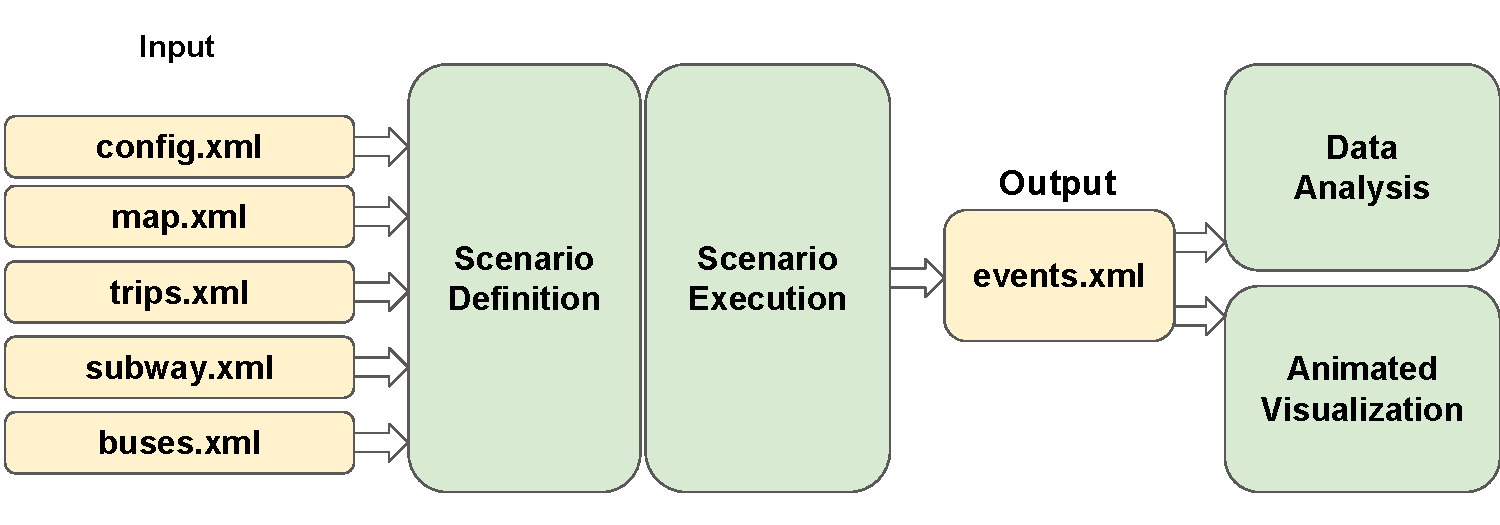
\includegraphics[width=1\textwidth]{figuras/chap-interscsimulator/components.pdf}
\caption{InterSCSimulator Components}
\label{fig:simComponents}
\end{figure}

The following sections will present each of the inputs, outputs, and components of the simulator.

\subsection{Inputs}

InterSCSimulator has three required XML files as input and other two optional files. The required files are:

\begin{itemize}

\item \textbf{config.xml} contains the path to the input and output files and the total simulation time.

\item \textbf{map.xml} has the digraph representing the road network of the simulated city. We used the map on the OpenStreetMap format in which the junctions are the vertices, and the streets are the links of the graph.

\item \textbf{trips.xml} defines the trips that must be simulated, each trip must determine its options such as origin, destination, start time, and travel mode.

\end{itemize}

The optional files are:

\begin{itemize}
    
\item \textbf{subway.xml} describes the city subway system as a graph which the stations are the vertices and the connection among the stations the edges.

\item \textbf{buses.xml} contains the bus lines of the city, including its name, interval, and bus stops sequences.

\end{itemize}

The map file is transformed in a digraph using the Digraph API of the Erlang language\footnote{Erlang Digraph API - \url{erlang.org/doc/man/digraph.html}}. Listing \ref{list:city} shows an example of a map used in the simulator.

\renewcommand{\thelstlisting}{\arabic{lstlisting}}
\lstset{language=XML}
\begin{lstlisting}[language=XML, caption=File describing the city road network, label=list:city, upquote=true]
<network>
 <nodes>
  <node id ="1" x="-46.65805" y="-23.58162" />
  <node id ="2" x="-46.65828" y="-23.58342" />
  <node id ="3" x="-46.65228" y="-23.59341" />
  <node id ="4" x="-46.63128" y="-23.51241" />
  <node id ="5" x="-46.59228" y="-23.54341" />
 </ nodes>
 <links>
  <link id="35985" from="1" to="2" length="100" freespeed="40" />
  <link id="35986" from="2" to="3" length="200" freespeed="40" />
  <link id="35987" from="3" to="1" length="80" freespeed="50" />
  <link id="35988" from="4" to="1" length="180" freespeed="50" />
  <link id="35989" from="1" to="5" length="30" freespeed="30" />
  <link id="35990" from="6" to="2" length="40" freespeed="50" />
  <link id="35991" from="7" to="2" length="50" freespeed="50" />
  <link id="35992" from="1" to="7" length="60" freespeed="40" />
  <link id="35988" from="3" to="6" length="180" freespeed="50" />
 </ links>
</network>
\end{lstlisting}

The map file has two section, the first describes the vertex of the graph, that are intersections among the cities roads. The vertex has three attributes, an Id, the latitude and the longitude. The second section contains all the edges of the graph, which represents a street stretch. The properties of the edges are its length, maximum speed, and capacity.

The trip file contains all the travels that must be simulated. Each travel has an origin and destination, the start time, and the travel model. A best path algorithm is used to define the travel path in the city graph. Listing  \ref{list:trips} presents an example of trips file with a set of travels.

\renewcommand{\thelstlisting}{\arabic{lstlisting}}
\lstset{language=XML}
\begin{lstlisting}[language=xml, caption=File containing the trips that will be simulated, label=list:trips, upquote=true]
<scsimulator_matrix>
 <trip origin="24751" dest="60613" start="2880" mode="car" />
 <trip origin="60613" dest="24791" start="6300" mode="car" />
 <trip origin="45110" dest="21990" start="1620" mode="car" />
 <trip origin="21090" dest="45110" start="6540" mode="car" />
 <trip origin="24751" dest="24650" start="3420" mode="car" />
 <trip origin="24650" dest="24751" start="5400" mode="car" />
 <trip origin="24751" dest="24650" start="6660" mode="car" />
 <trip origin="24650" dest="24751" start="8550" mode="walk" />
 <trip origin="24751" dest="24751" start="2370" mode="car" />
 <trip origin="24751" dest="24751" start="4440" mode="car" />
 <trip origin="24751" dest="60658" start="2880" mode="car" />
 <trip origin="60658" dest="24791" start="4320" mode="car" />
 <trip origin="24751" dest="41594" start="6840" mode="walk" />
 <trip origin="25822" dest="27925" start="7920" mode="car" />
 <trip origin="27925" dest="66111" start="5760" mode="car" />
 <trip origin="66111" dest="27925" start="6480" mode="car" />
 <trip origin="24751" dest="33026" start="4230" mode="car" />
</scsimulator_matrix>
\end{lstlisting}

It is also possible to simulate multimodal travels. For example, a person can walk until a bus stop, take a bus to a subway station, and then go walking from other metro station until its work. Listing \ref{list:multi_trips} presents examples of multimodal travels.

\renewcommand{\thelstlisting}{\arabic{lstlisting}}
\lstset{language=XML}
\begin{lstlisting}[language=xml, caption=Multi-Trip file, label=list:multi_trips, upquote=true]
<multi_trip name="1"  count="45" start="43201" mode="bus">
  <trip origin="25298" dest="17409" mode="walk"/>
  <trip origin="17409" dest="11072" line="8020-10-0" mode="bus"/>
  <trip origin="11072" dest="30469" line="675N-10-0" mode="bus"/>
  <trip origin="30469" dest="30469" mode="walk"/>
</multi_trip>
<multi_trip name="3" count="82" start="45001" mode="metro">
  <trip origin="41972" dest="44116" mode="walk"/>
  <trip origin="44116" dest="25781" mode="metro"/>
  <trip origin="25781" dest="30165" mode="walk"/>
</multi_trip>
<multi_trip name="4" count="37" start="61201" mode="metro">
  <trip origin="31468" dest="29513" mode="walk"/>
  <trip origin="29513" dest="28267" mode="metro"/>
  <trip origin="28267" dest="60642" mode="walk"/>
</multi_trip>
\end{lstlisting}


The Config file defines some parameters to the simulator such as the total time of the simulation, the path to the input and output files and what analyses will be executed in the final of the simulation. Listing \ref{list:config} presents an example of this file.

\renewcommand{\thelstlisting}{\arabic{lstlisting}}
\lstset{language=XML}
\begin{lstlisting}[language=xml, caption=File with the simulator configurations, label=list:config, upquote=true]
<scsimulator_config>
    <config trip_file="path_to_trip_file" />
    <config map_file="path_to_map_file" />
    <config bus_file="path_to_bus_file" />
    <config subway_file="path_to_subway_file" />
    <config simulation_time="86400" />
    <outputs>
        <chart name="mostUsedRoads" />
        <chart name="meanVelocityHour" />
        <chart name="tripTimeByMode" />
    </outputs>
</scsimulator_config>
\end{lstlisting}

The subway file defines the subway graph of the simulated city which has two sections. The first describes the subway stations and the second the connections among the stations. Listing \ref{list:subway} presents an example of the definition of a subway line in the input file.

\renewcommand{\thelstlisting}{\arabic{lstlisting}}
\lstset{language=XML}
\begin{lstlisting}[language=xml, caption=File with the definition of the city subway graph, label=list:subway, upquote=true]
<metro>
  <stations>
    <station name="Vila Prudente" idNode="252018921" />
    <station name="Tamanduatei" idNode="674412889" />
    <station name="Sacoma" idNode="2533391001" />
    <station name="Alto Do Ipiranga" idNode="4443113954" />
    <station name="Santos-imigrantes" idNode="1484829870" />
    <station name="Chacara Klabin" idNode="922094745" />
    <station name="Ana Rosa" idNode="467744160" />
    <station name="Paraiso" idNode="459347687" />
    <station name="Brigadeiro" idNode="856727276" />
    <station name="Trianon-masp" idNode="2021000708" />
    <station name="Consolacaoo" idNode="1819616337" />
    <station name="Clinicas" idNode="1952545109" />
    <station name="Sumare" idNode="466808387" />
    <station name="Vila Madalena" idNode="1415720983" />
  </stations>

  <links>
    <link idOrigin="674412889" idDestination="252018921" />
    <link idOrigin="2533391001" idDestination="674412889" />
    <link idOrigin="4443113954" idDestination="2533391001" />
    <link idOrigin="1484829870" idDestination="4443113954" />
    <link idOrigin="922094745" idDestination="1484829870" />
    <link idOrigin="467744160" idDestination="922094745" />
    <link idOrigin="459347687" idDestination="467744160" />
    <link idOrigin="856727276" idDestination="459347687" />
    <link idOrigin="2021000708" idDestination="856727276" />
    <link idOrigin="1819616337" idDestination="2021000708" />
    <link idOrigin="1952545109" idDestination="1819616337" />
    <link idOrigin="466808387" idDestination="1952545109" />
    <link idOrigin="1415720983" idDestination="466808387" />
  </links>
</metro>
\end{lstlisting}

The buses file defines the bus lines in the simulated city. Each bus line has the following attributes: \textbf{Id} is the name of the line; \textbf{interval} is the dispatch time interval of the buses of the line; \textbf{start\_time} is the bus first dispatch time of the day; \textbf{stops} is the list of bus stops whose the bus must stop to load or unload passengers. Listing \ref{list:buses} presents an example of the definition of bus lines in the simulator.

\renewcommand{\thelstlisting}{\arabic{lstlisting}}
\lstset{language=XML}
\begin{lstlisting}[language=xml, caption=Definition of the city buses, label=list:buses, upquote=true]

<scsimulator_buses>
    <bus id="1016-10-0" interval="1800" start_time="18000" stops="507969889,2390204059,507969889,1400446171" />
    <bus id="1016-10-1" interval="1800" start_time="18000" stops="2396517544,163220296,2390192810,2390192798
    " />
    <bus id="1017-10-0" interval="1800" start_time="18000" stops="832264854,1758396031,832264854,2448473366" />
    <bus id="1017-10-1" interval="1800" start_time="18000" stops="934050061,2109902387,2448473366,832264854" />
    <bus id="1018-10-0" interval="1800" start_time="18000" stops="2116463109,2390204059,507969889,2390204059" />
    <bus id="1018-10-1" interval="1800" start_time="18000" stops="2520196336,507969946,410243261,410243260" />
    <bus id="1024-10-0" interval="1800" start_time="18000" stops="934050061,1430544803,917144410,1430544803,917144410" />
    <bus id="1025-10-0" interval="1800" start_time="18000" stops="934050061,1430544803,917144410,1430544803" />
    <bus id="106A-10-0" interval="1800" start_time="18000" stops="2390339037,1709028082,185795118,929591881" />
</scsimulator_buses>

\end{lstlisting}

\subsection{Scenario Definition}

The Scenario Definition component parses the input file and creates the simulation scenario. Additionally, it creates all the management Erlang actors and sets all the parameters of the simulation such as the simulation time and the output path. The most critical actors created in this phase are the \textbf{travel manager}, which generates the people actors during the simulation, \textbf{subway manager} which represents the subway system of the city, \textbf{city manager} which describes the road network of the town, and the \textbf{output manager} which saves all the simulation events to the log file.

In this phase are also calculated the best path to all the car and pedestrian travels. It is made before the simulation because it is a costly operation and if it was executed during the simulation could waste a lot of processing time.

\subsection{Simulation Execution}
\label{sub:execucao}

In the execution of the simulator, the most important actions are the movement of people on foot, by car, or by public transportation. Each person of the simulation make an action (or event) and then schedules its next movement. The movement depends on the transportation modal of the person. In the following, we describe the main events that a person can execute during the simulation.

\begin{itemize}

\item \textbf{Start Travel: } When the simulation time is equal to the start time of the travel configuration, an agent is created to simulate that travel. Independently of the transportation mode. In this event, the agent goes to the first link of its path.

\item \textbf{Move: } If an agent is moving on foot or car when it leaves a link and enters in another one, it is generated a move event. In this event, it is calculated the time that the agent will require to pass through the link. Walks and car travels are a succession of move events.

\item \textbf{Move Bus:} When an agent arrives at a bus station, it waits until a bus of the line that it is waiting arrives. When the bus arrives, the agent enters the bus and generates a move bus event. After, the agent moves with the bus until its bus stop destination.

\item \textbf{Move Subway: } If an agent will travel by subway when it arrives at the subway station, it informs the SubwayManager their origin and destination stations. The SubwayManager calculates the time in which the agent will spend in the subway system and notifies the agent. 

\item \textbf{Arrival: } When the agent arrives at its final destination, it creates an arrival event that saves the attributes of the travel in the output file such as the total time, distance, and cost. After this event, the agent is removed from the simulation.

\end{itemize}

The execution of the events is based on the models described in Section \ref{sub:modelo}. All the events are saved on the simulator output file in chronological order and have common attributes such as simulation tick, link, type, and id of the agent which executed the event.

\subsection{Outputs}
\label{sub:saida}

As output, InterSCSimulator generates an XML or CSV file with all the events occurred during the simulation. The possible events are the ones described in the previous section. Listing \ref{list:csv_output} presents a stretch of the file with a simulation output.

\lstset{language=XML}
\begin{lstlisting}[caption=CSV output file, label=list:csv_output]
192;arrival;8062_65;102388;126;616
200;arrival;8062_74;102388;126;616
228;arrival;8062_38;102388;126;616
235;arrival;8000_50;106030;186;1542
244;arrival;8062_37;102388;126;616
257;arrival;49_10;48743;157;807
257;arrival;49_17;48743;157;807
258;arrival;8062_20;102388;126;616
259;arrival;2280_15;13694;91;407
269;arrival;3241_72;42753;144;1668
\end{lstlisting}

In Listing \ref{list:csv_output} the first four elements are common to all events which are the simulation tick, the event, the agent id, and the link where the event occurred. Depending on the event, it could have more elements, such as the arrival event that also saves the total distance and the total time of the travel.

To generate the XML file, we used the MATSim format, allowing the usage of OTFVis\footnote{OTFVis --- \url{matsim.org/docs/extensions/otfvis}}, a tool to generate an animated visualization of the simulation. Listing \ref{list:xml_output} presents a stretch of the file with the XML output.

\lstset{language=XML}
\begin{lstlisting}[language=xml, caption=XML output file, label=list:xml_output]
<events version="1.0">
  <event time="28" type="departure" person="p1" link="1425"  />
  <event time="28" type="entered link" person="p1" link="15" vehicle="car1" />
  <event time="32" type="entered link" person="p1" link="13" vehicle="car1" />
  <event time="54" type="entered link" person="p1" link="16" vehicle="car1" />
  <event time="62" type="entered link" person="p1" link="36" vehicle="car1" />
  <event time="78" type="entered link" person="p1" link="21" vehicle="car1" />
  <event time="96" type="entered link" person="p1" link="42" vehicle="car1" />
  <event time="110" type="entered link" person="p1" link="57" vehicle="car1" />
  <event time="114" type="entered link" person="p1" link="72" vehicle="car1" />
  <event time="118" type="entered link" person="p1" link="67" vehicle="car1" />
  <event time="125" type="arrival" person="p1" vehicle="car1" link="88" trip_time="191" distance="2634" />
</events>
\end{lstlisting}


\subsection{Simulation Visualization}

Using the output data, it is possible to generate different visualizations of the simulation results. For example, it is possible to create an animated visualization of the simulation events. This visualization shows the city road network and the cars moving in the city. Figure \ref{fig:sao_paulo_map} presents the visualization of one simulation in the city of S\~ao Paulo. Each green point in the figure is a car moving in the city graph.

\begin{figure}[!htb]
\centering
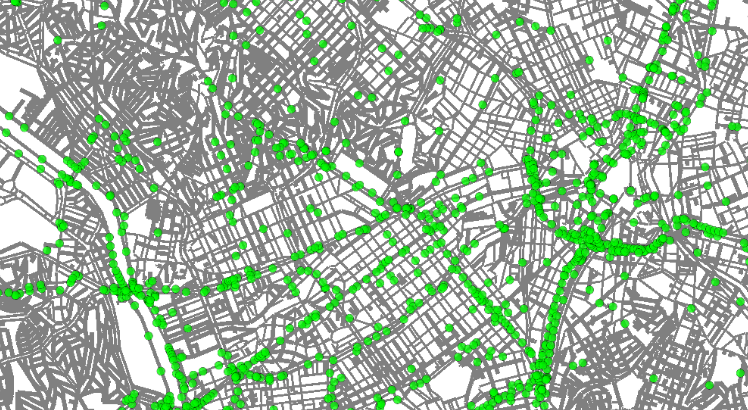
\includegraphics[width=0.9\textwidth]{figuras/chap-interscsimulator/mapa.png}
\caption{S\~ao Paulo Simulation}
\label{fig:sao_paulo_map}
\end{figure}

To show that InterSCSimulator works in any map generated from the OSM, we also made a simple simulation using the map of New York. Figure \ref{fig:newYork} presents the visualization of this simulation using OTFVis.

\begin{figure}[!htb]
\centering
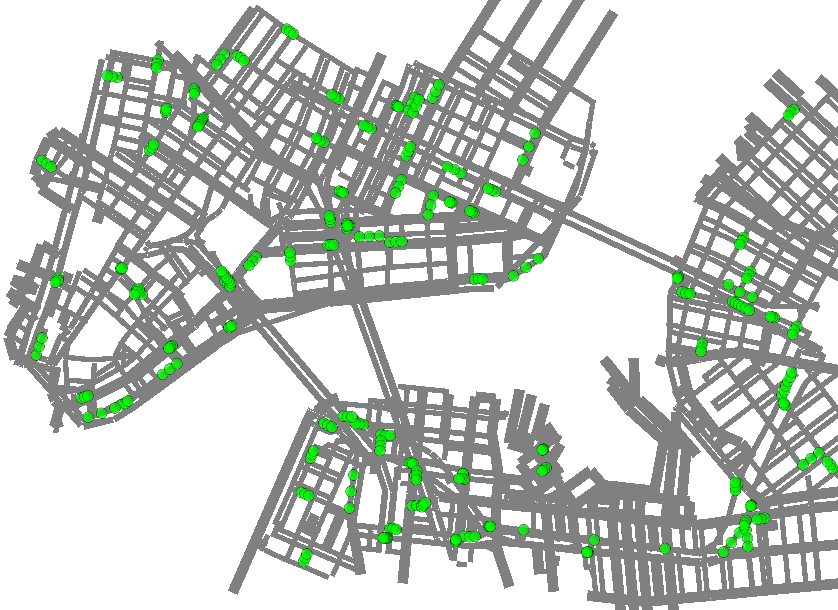
\includegraphics[width=0.7\textwidth]{figuras/mapaNy.png}
\caption{New York Simulation}
\label{fig:newYork}
\end{figure}

Despite that OTFVis is capable of simulating large simulations with more than 50 thousand actors at the same time, it does not have the same scalability as InterSCSimulator. Therefore, it is necessary more research allow the visualization of a very-large simulation in a large graph such as S\~ao Paulo road network.

Besides the animated visualization, we also created a component that executes scripts written in R language to perform statistical analyses with the output data of the simulator. These scripts generate a series of charts such as the mean speed of the cars during the simulation time, the most used links in the simulation, and the mean time of the travels by the transportation mode. Figure \ref{fig:chart_example} shows a chart generated by an R script which shows the 10 most used links during the simulation.

\begin{figure}[!htb]
\centering
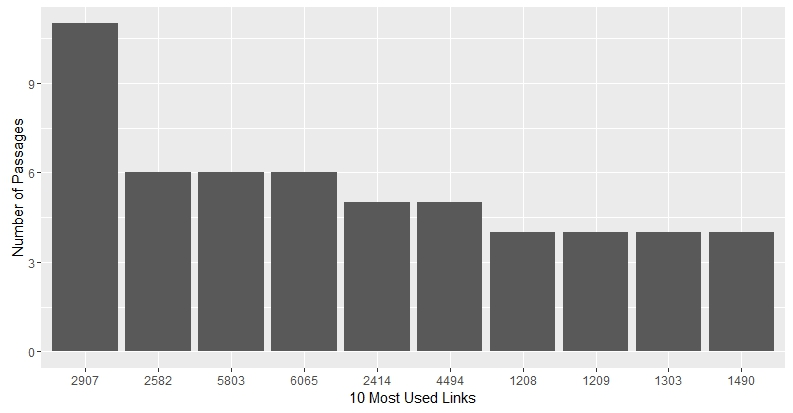
\includegraphics[width=0.8\textwidth]{figuras/chart_top_ten.jpeg}
\caption{Most used links in the simulation}
\label{fig:chart_example}
\end{figure}

Figure \ref{fig:chart_example2} presents another example of a chart generated using the simulation output data. This chart presents the mean travel time by the different type of travels such as agents going to work, to home, or going to hospitals.

\begin{figure}[!htb]
\centering
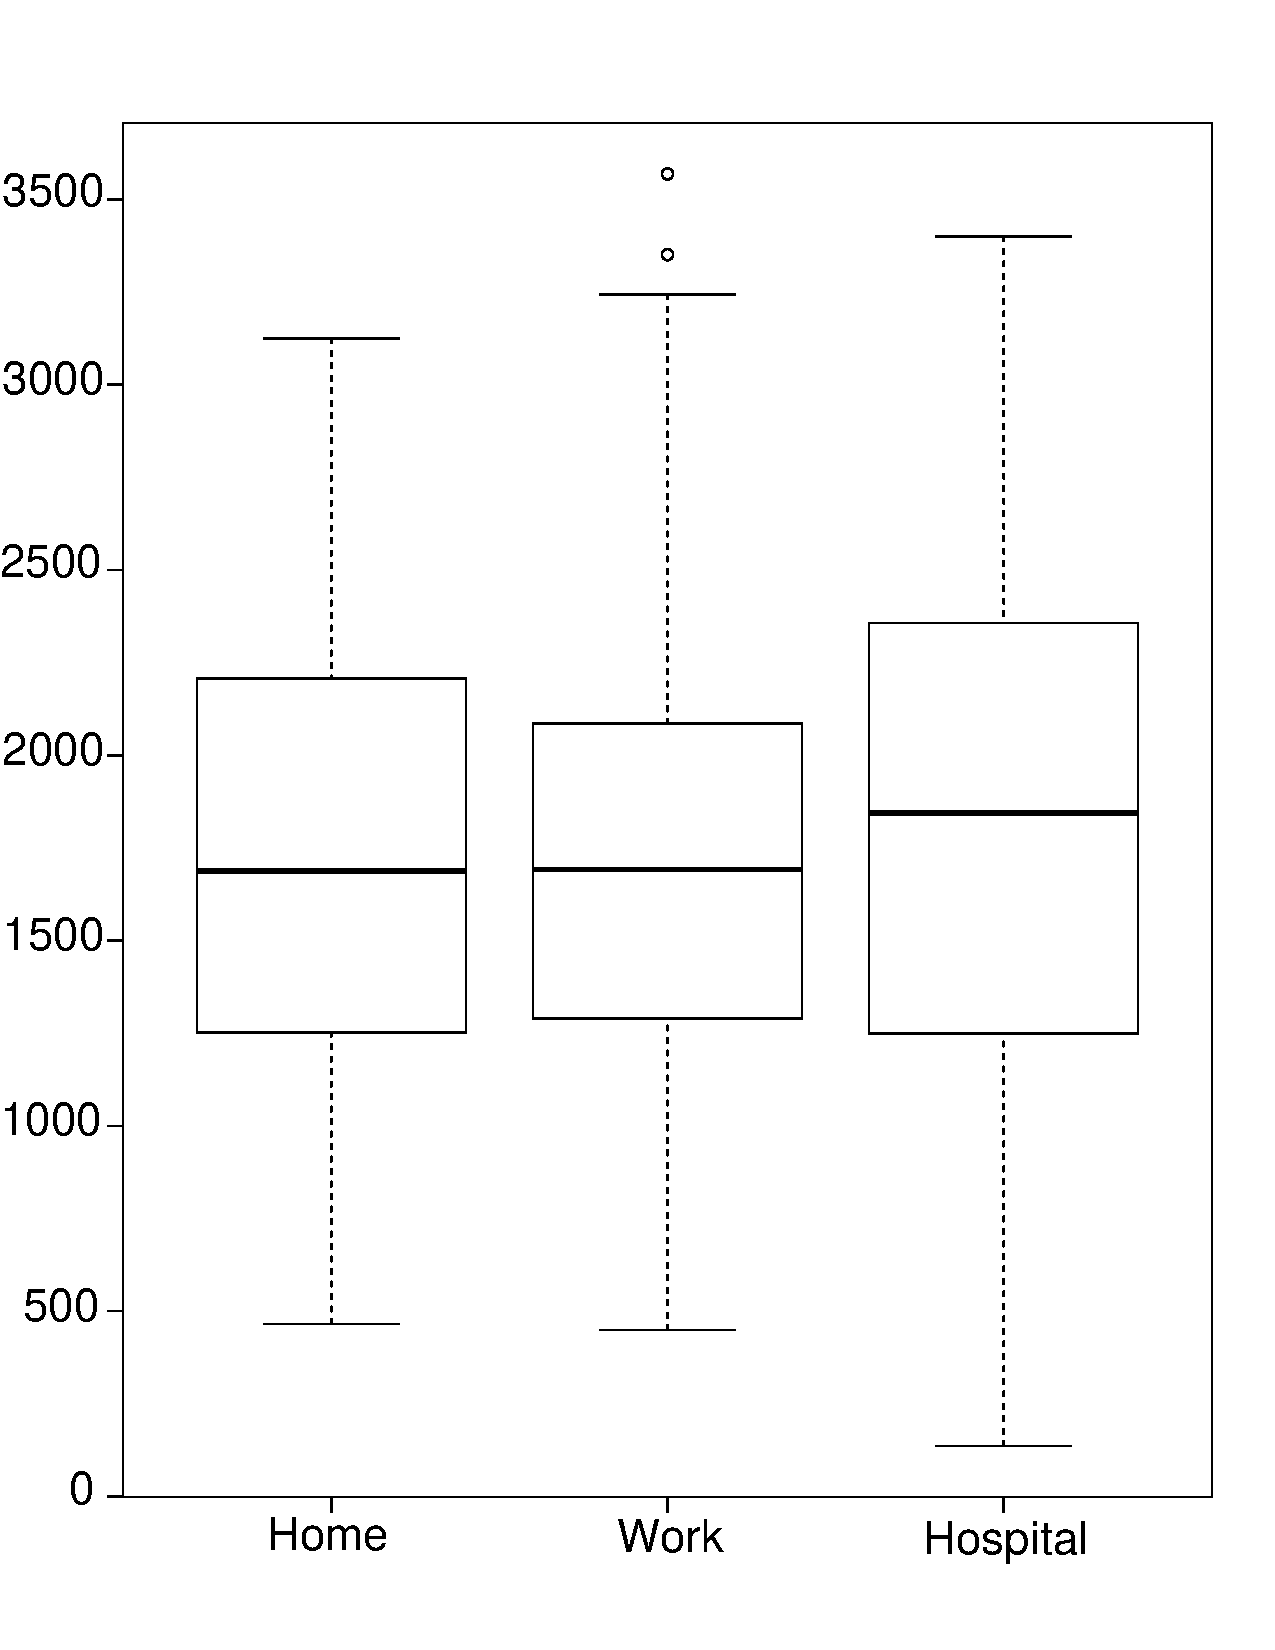
\includegraphics[width=0.6\textwidth]{figuras/mode_trip.pdf}
\caption{Mean travel time by travel type}
\label{fig:chart_example2}
\end{figure}


\section{Other Simulations}
\label{sec:outros}

Besides the models described in this Chapter, we also implemented other components of Smart Cities applications such as:

\begin{itemize}

    \item \textbf{Parking Spots:} We also developed the simulation of parking spots, which allow the configuration of a car travel that the person must find a free place to park the car. The idea of this simulation was to verify the impact in the city traffic of using a Smart Parking application, helping drivers to find the closest free parking spot.
 
    \item \textbf{Sensors:} The simulator enables the definition of a set of sensors which generates data in a time interval. These actors allow the simulation of different type of sensors such as air pollution, noise, traffic counters, and humidity. The simulation of sensors enables tests and experiments of Smart City applications and platforms.
    
    \item \textbf{Locations:} It is possible to simulate locations in the simulator. These locations can generate random travels in the city using a statistical distribution. The idea of this model is to reproduce places in the city that can spawn traffic such as stadiums, shopping centers, and large condominiums.
    
    \item \textbf{Events:} The simulator allows the simulation of events in the city streets such as an accident that interferes in the flow of vehicles or streets closure in a weekend for leisure. The idea of simulating events is to evaluate how an event impacts the traffic of the city.
    
\end{itemize}


\section{Simulator Architecture Evolution}
\label{sec:evolucao}

Achieve the current scalability of the simulator was a big challenge. We had to develop different algorithms and use many data structures during the simulator implementation. This section presents the most significant modifications to the simulator architecture to improve the execution time and memory usage. The most significant improvements were in the city graph representation and the actor's creation.

\subsection{City Graph Representation}

To manipulate the city graph, we use the Erlang Digraph API\footnote{Digraph API -- http://erlang.org/doc/man/digraph.html} which facilitates a lot the creation of graphs and the execution of many algorithms such as the best path and minimal spanning tree.

In the first version of the simulator, we maintained the city graph in a unique Erlang actor. When a car entered a link, it must send a message to the graph actor and waits for the execution of the traffic model to get the time that it took to go through the street. This model worked but had a very high execution time, because this central actor was a bottleneck in the simulator architecture. We did not execute scalability tests in this version because we could simulate at most 50,000 agents in this version of the simulator.

The first solution to this problem was creating an independent actor to each vertex in the graph. In the second version, each actor had the id of the vertex and a dictionary\footnote{Erlang Dictionary -- http://erlang.org/doc/man/dict.html} with all the links to the adjacent vertex. This dictionary stored the attributes of the link such as its length, capacity, and the current number of cars in the link. This version increased a lot the use of memory to store the city graph but lowered the execution time of the simulator. With this version, it was possible to execute simulations with more than 4 million actors in a single simulation. Figure \ref{fig:execution_time} shows the execution time of this version of the simulator using a S\~ao Paulo scenario with 1, 2, 3, and 4 million cars.

Although the second version of the simulator improved a lot the simulator execution time, the architecture of the simulator with an Erlang actor to each vertex of the graph was using much memory and when the traffic was very congested, a number of vertex, mainly the ones that represented big avenues in the city, the execution time of the simulation increased a lot. To solve this problem, we used the Erlang ETS (Erlang Term Storage) Tables \cite{aronis2017shared}.

The ETS Table is an in-memory store object available in the Erlang Virtual Machine. An ETS Table is capable of storing large amounts of objects with a constant time data access. All the Erlang actors can access and update an ETS table that is running in the Erlang VM. To avoid concurrency problems, the ETS API provides a series of atomic operations such as increment, decrements, exclusion of lists, and value update.

The third, and current, version of the simulator uses an ETS table to store the city graph. In this version, the digraph API is used only to calculate the travel paths. The models use the ETS that has all the vertex and links of the graph. Using the ETS there is no bottleneck in the simulator, the only problem that can occur is if two or more vehicles try to enter in the same link at the same moment. If this occurs, the cars will have to wait for the update in the ETS table from the other cars. The use of ETS table improved the execution time of the simulator almost three times. Figure \ref{fig:execution_time} shows the execution time of this version of the simulator using the same scenarios of the previous Figure.

\begin{figure}[!htb]
\centering
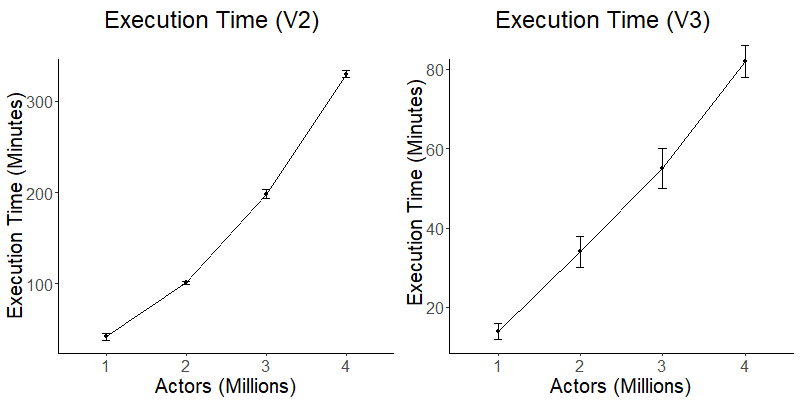
\includegraphics[width=1.0\textwidth]{figuras/chap-interscsimulator/execution_time.png}
\caption{Execution Time of InterSCSimulator V2 and V3 (ATUALIZAR PARA OS GRÁFICOS DA NOVA VERSÂO)}
\label{fig:execution_time}
\end{figure}

\subsection{Actors Creation}

In the InterSCSimulator, an Erlang actor performs each simulated travel. Therefore, if a simulation has 10 million travels, 10 million Erlang actors are created during the simulation. In the first version of the simulator, all the actors were created during the simulation. It was not a problem because the simulator maximum scalability was 50 thousand actors.

However, in the second version of the simulator, the scale increased a lot and the creation of the actors was a bottleneck in the simulation and we found a bug in the Sim-Diasca simulator that made the creation of actor very slow. To minimize this problem, we decided to create all the actors before the simulation start. This approach solved the scalability problem but increased the memory used by the simulator. Figure \ref{fig:memory_used} shows the memory used to execute the simulations in this version of the simulator.

In the third version, the Sim-Diasca developers solved the problem in the actor creation and released a new version of the simulator. Therefore, we could return to the first approach and create the actors during the simulation. Along with other improvements in the simulator, including the ETS tables, the third version of the simulator uses almost five times less memory to execute. Figure \ref{fig:memory_used} shows the memory used to execute the simulations in this version of the simulator.

\begin{figure}[!htb]
\centering
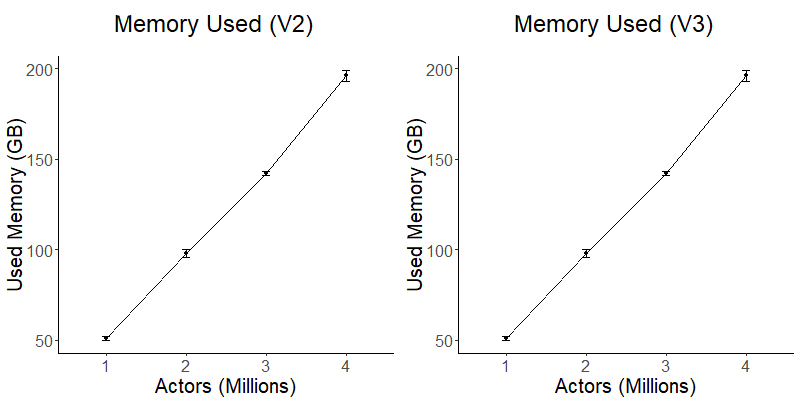
\includegraphics[width=1.0\textwidth]{figuras/chap-interscsimulator/memory_used.png}
\caption{Memory Used in InterSCSimulator V2 and V3(ATUALIZAR PARA OS GRÁFICOS DA NOVA VERSÂO)}
\label{fig:memory_used}
\end{figure}